\chapter{Background}
\label{ch:background}

This chapter provides the shared background for the rest of the thesis.
The five systems presented in later chapters touch different layers of the LLM serving stack, from decoding algorithms (\Cref{ch:specinfer,ch:suffixdecoding}) and cluster-level resource allocation (\Cref{ch:flexllm}) down to the GPU kernels that every layer above ultimately runs on (\Cref{ch:fastkernels,ch:kernelseek}).
Rather than repeat the same material in each chapter, we collect it here: how large language models are structured and why autoregressive inference is expensive (\Cref{background:sec:llm}), how production serving systems organize that inference (\Cref{background:sec:serving}), how speculative decoding converts sequential generation into parallel verification (\Cref{background:sec:specdec}), how parameter-efficient finetuning is offered alongside inference on shared platforms (\Cref{background:sec:peft}), what agentic workloads look like and why they stress serving systems (\Cref{background:sec:agents}), how GPUs execute kernels and why writing fast ones is hard (\Cref{background:sec:gpu}), and how LLM agents are being applied to the problem of writing those kernels (\Cref{background:sec:kernelagents}).

The treatment is deliberately selective. Each section goes only as deep as the later chapters require, and it ends by positioning the corresponding chapter against the work it builds on. Each later chapter then adds its own focused background and a related-work section that discusses its immediate neighbors in more detail; this chapter is the map, and the chapters are the territory. We close with a short summary (\Cref{background:sec:summary}) that ties the sections back to the thesis statement.

\section{Large Language Models and Autoregressive Inference}
\label{background:sec:llm}

\subsection{The Transformer Decoder}
\label{background:subsec:transformer}

Nearly every large language model (LLM) deployed today is a decoder-only Transformer~\cite{vaswani,radford2019language,brown2020language}.
The model maps a sequence of discrete tokens to a probability distribution over the next token.
An \emph{embedding} table converts each token identifier into a vector of dimension $d$ (the hidden size), and a stack of $L$ identical \emph{decoder layers} transforms the resulting sequence of vectors.
A final linear projection, the \emph{language-model head}, maps the hidden state at each position back onto the vocabulary (typically 32K--256K entries), and a softmax turns the resulting logits into a distribution.

Each decoder layer has two sublayers wrapped in residual connections and normalization.
The first is \emph{multi-head self-attention}.
For every token the layer computes a query $q$, a key $k$, and a value $v$ by linear projection of the token's hidden state; the attention output for a token at position $t$ is a weighted average of the values of all positions $\le t$, with weights $\mathrm{softmax}(q_t k_j^{\top}/\sqrt{d_h})$ over $j \le t$, computed independently in each of $H$ heads of dimension $d_h = d/H$.
The causal mask (positions $j > t$ are excluded) is what makes the model a left-to-right language model, and it is also what allows the keys and values of earlier tokens to be cached and reused, as we discuss below.
Multi-query and grouped-query attention~\cite{shazeer2019fast,ainslie2023gqa} share key and value projections across groups of query heads to reduce the size of this cache; most recent open models (LLaMA-3, Qwen-2.5, and later~\cite{llama3,qwen2025qwen25technicalreport}) use grouped-query attention.
The second sublayer is a position-wise \emph{feed-forward network} (FFN), typically two or three linear projections with a nonlinearity between them, applied identically to every token.
For a dense model the parameter count is dominated by the attention projections and the FFN, and the compute of a forward pass is dominated by the corresponding matrix multiplications; for a model with $N$ parameters, processing one token costs roughly $2N$ floating-point operations plus the attention term, which grows with the sequence length~\cite{kaplan2020scaling,pope2023efficiently}.

\paragraph{Emerging operators.}
The dense Transformer is no longer the only architecture that serving systems must support, and the variants matter for this thesis because they are precisely the operators for which hand-optimized kernels lag the furthest behind (\Cref{background:sec:gpu}).
\emph{Mixture-of-experts} (MoE) layers~\cite{shazeer2017outrageously,fedus2022switch} replace the single FFN with many expert FFNs and a router that sends each token to a small subset of them; models such as Mixtral, DeepSeek-V3, LLaMA-4, and Qwen-3~\cite{jiang2024mixtral,deepseekai2024deepseekv3,llama4,yang2025qwen3technicalreport} decouple parameter count from per-token compute in this way, at the price of data-dependent routing, load imbalance across experts, and irregular memory access.
\emph{Linear attention}~\cite{katharopoulos2020transformers} and \emph{state-space models} such as Mamba and Mamba-2~\cite{gu2023mamba,mamba2}, together with hybrids such as gated delta networks~\cite{yang2025gated}, replace the softmax attention over the full history with a recurrent state of fixed size, trading the quadratic cost and growing cache of attention for a scan or chunked recurrence whose efficient implementation looks nothing like a matrix multiplication.
Low-bit quantization of weights and activations~\cite{xiao2022smoothquant,frantar2023gptq,dettmers2022gpt3} adds yet another family of operators (mixed-precision GEMMs, dequantization fused into matrix multiplies) with their own kernel requirements.
Each of these operators is a point where the architecture has moved faster than the kernels, a theme to which \Cref{ch:fastkernels,ch:kernelseek} return.

\subsection{Autoregressive Generation}
\label{background:subsec:autoregressive}

An LLM is used by giving it a \emph{prompt}, a sequence of tokens $x_1, \ldots, x_m$, and asking it to generate a continuation.
Generation is \emph{autoregressive}: the model produces one token at a time, and each new token is conditioned on the prompt and all previously generated tokens,
\[
x_{t+1} \sim P(x \mid x_1, \ldots, x_t; \Theta),
\]
until it emits an end-of-sequence token or reaches a length limit.
How the next token is drawn from the distribution is a choice of the application.
\emph{Greedy decoding} takes the most probable token.
\emph{Stochastic decoding} samples from the distribution, usually after reshaping it with a temperature and truncating it with top-$k$ or nucleus (top-$p$) sampling~\cite{holtzman2020curious}; chat and agentic deployments use both modes, and any acceleration technique that claims to be lossless must therefore preserve the output distribution in both cases (\Cref{background:sec:specdec}).

Because every token depends on the one before it, generation for a single request is inherently sequential: a request that produces $n$ output tokens requires $n$ dependent forward passes through the full model.
This is the central inefficiency that \Cref{ch:specinfer,ch:suffixdecoding} attack, and the rest of this section explains where it comes from and why it is so costly.

\paragraph{Prefill and decode.}
Serving systems split the processing of a request into two phases~\cite{yu2022orca,agrawal2023sarathi,miao2023towards}.
During \emph{prefill}, the model processes all $m$ prompt tokens in a single forward pass; the matrix multiplications see $m$ rows at once, so prefill is compute-intensive and makes good use of the GPU.
During \emph{decode}, the model processes exactly one new token per forward pass for each request (\Cref{background:fig:decoding:incremental}).
A decode step touches every parameter of the model to produce a single row of output per request, so its computational intensity is orders of magnitude lower than prefill, and its latency per step sets the latency per output token that users perceive.
The two phases have such different characteristics that recent systems schedule them differently or even run them on different GPUs (\Cref{background:sec:serving}).

\begin{figure}[t]
    \centering
    \begin{subfigure}[t]{0.41\linewidth}
        \centering
        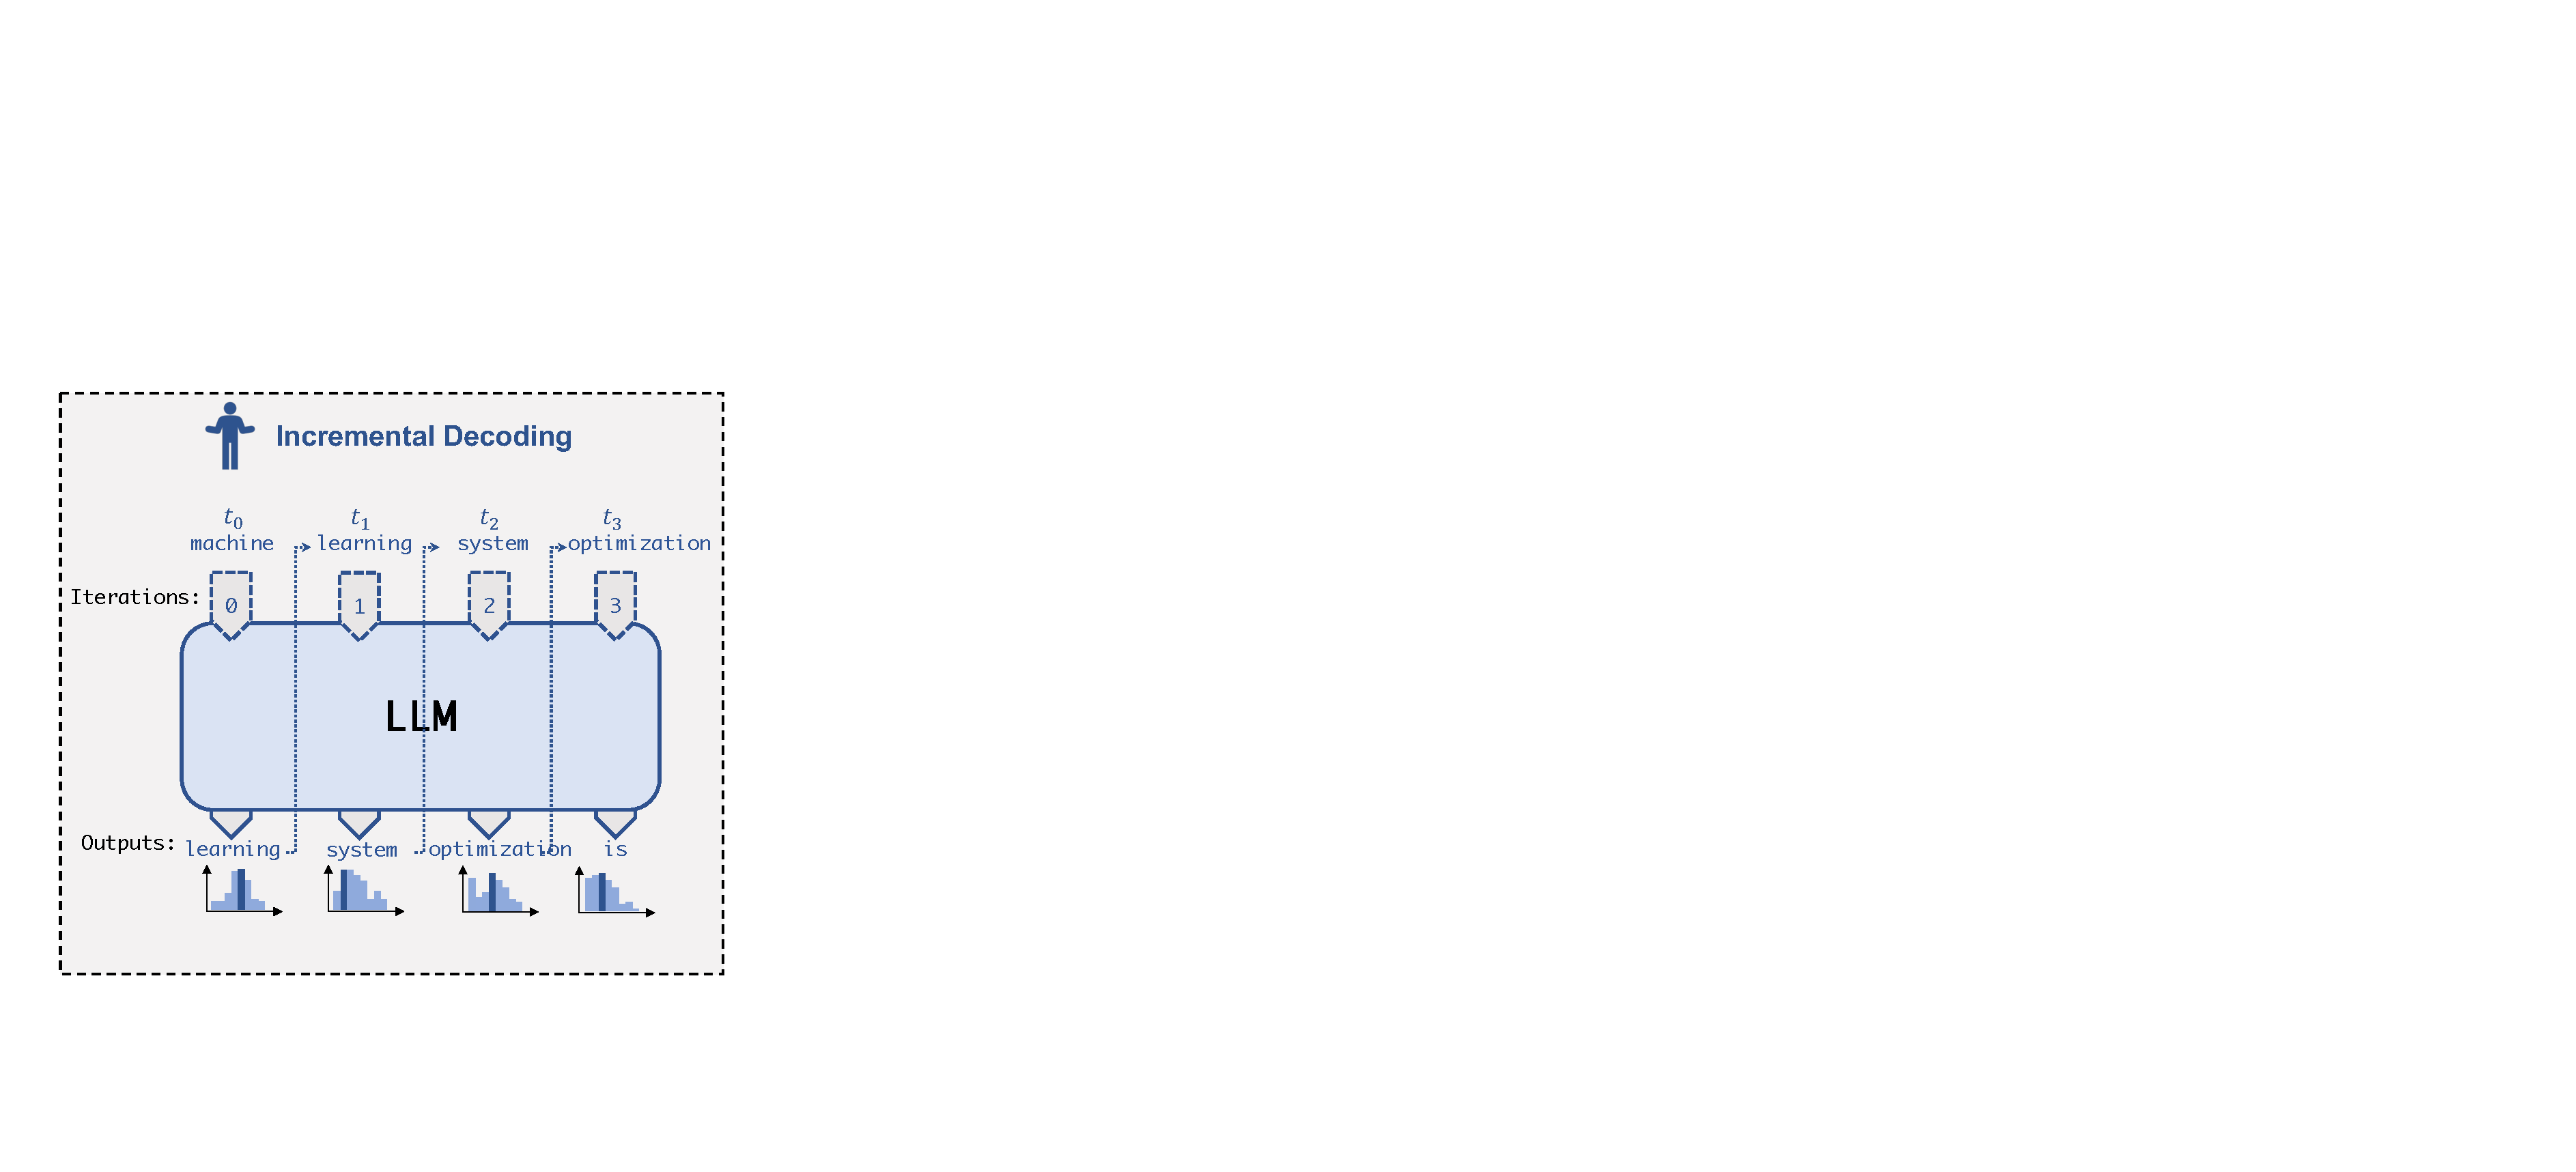
\includegraphics[width=\linewidth]{figures/specinfer/existing_overview6a4}
        \caption{Incremental decoding.}
        \label{background:fig:decoding:incremental}
    \end{subfigure}
    \hfill
    \begin{subfigure}[t]{0.56\linewidth}
        \centering
        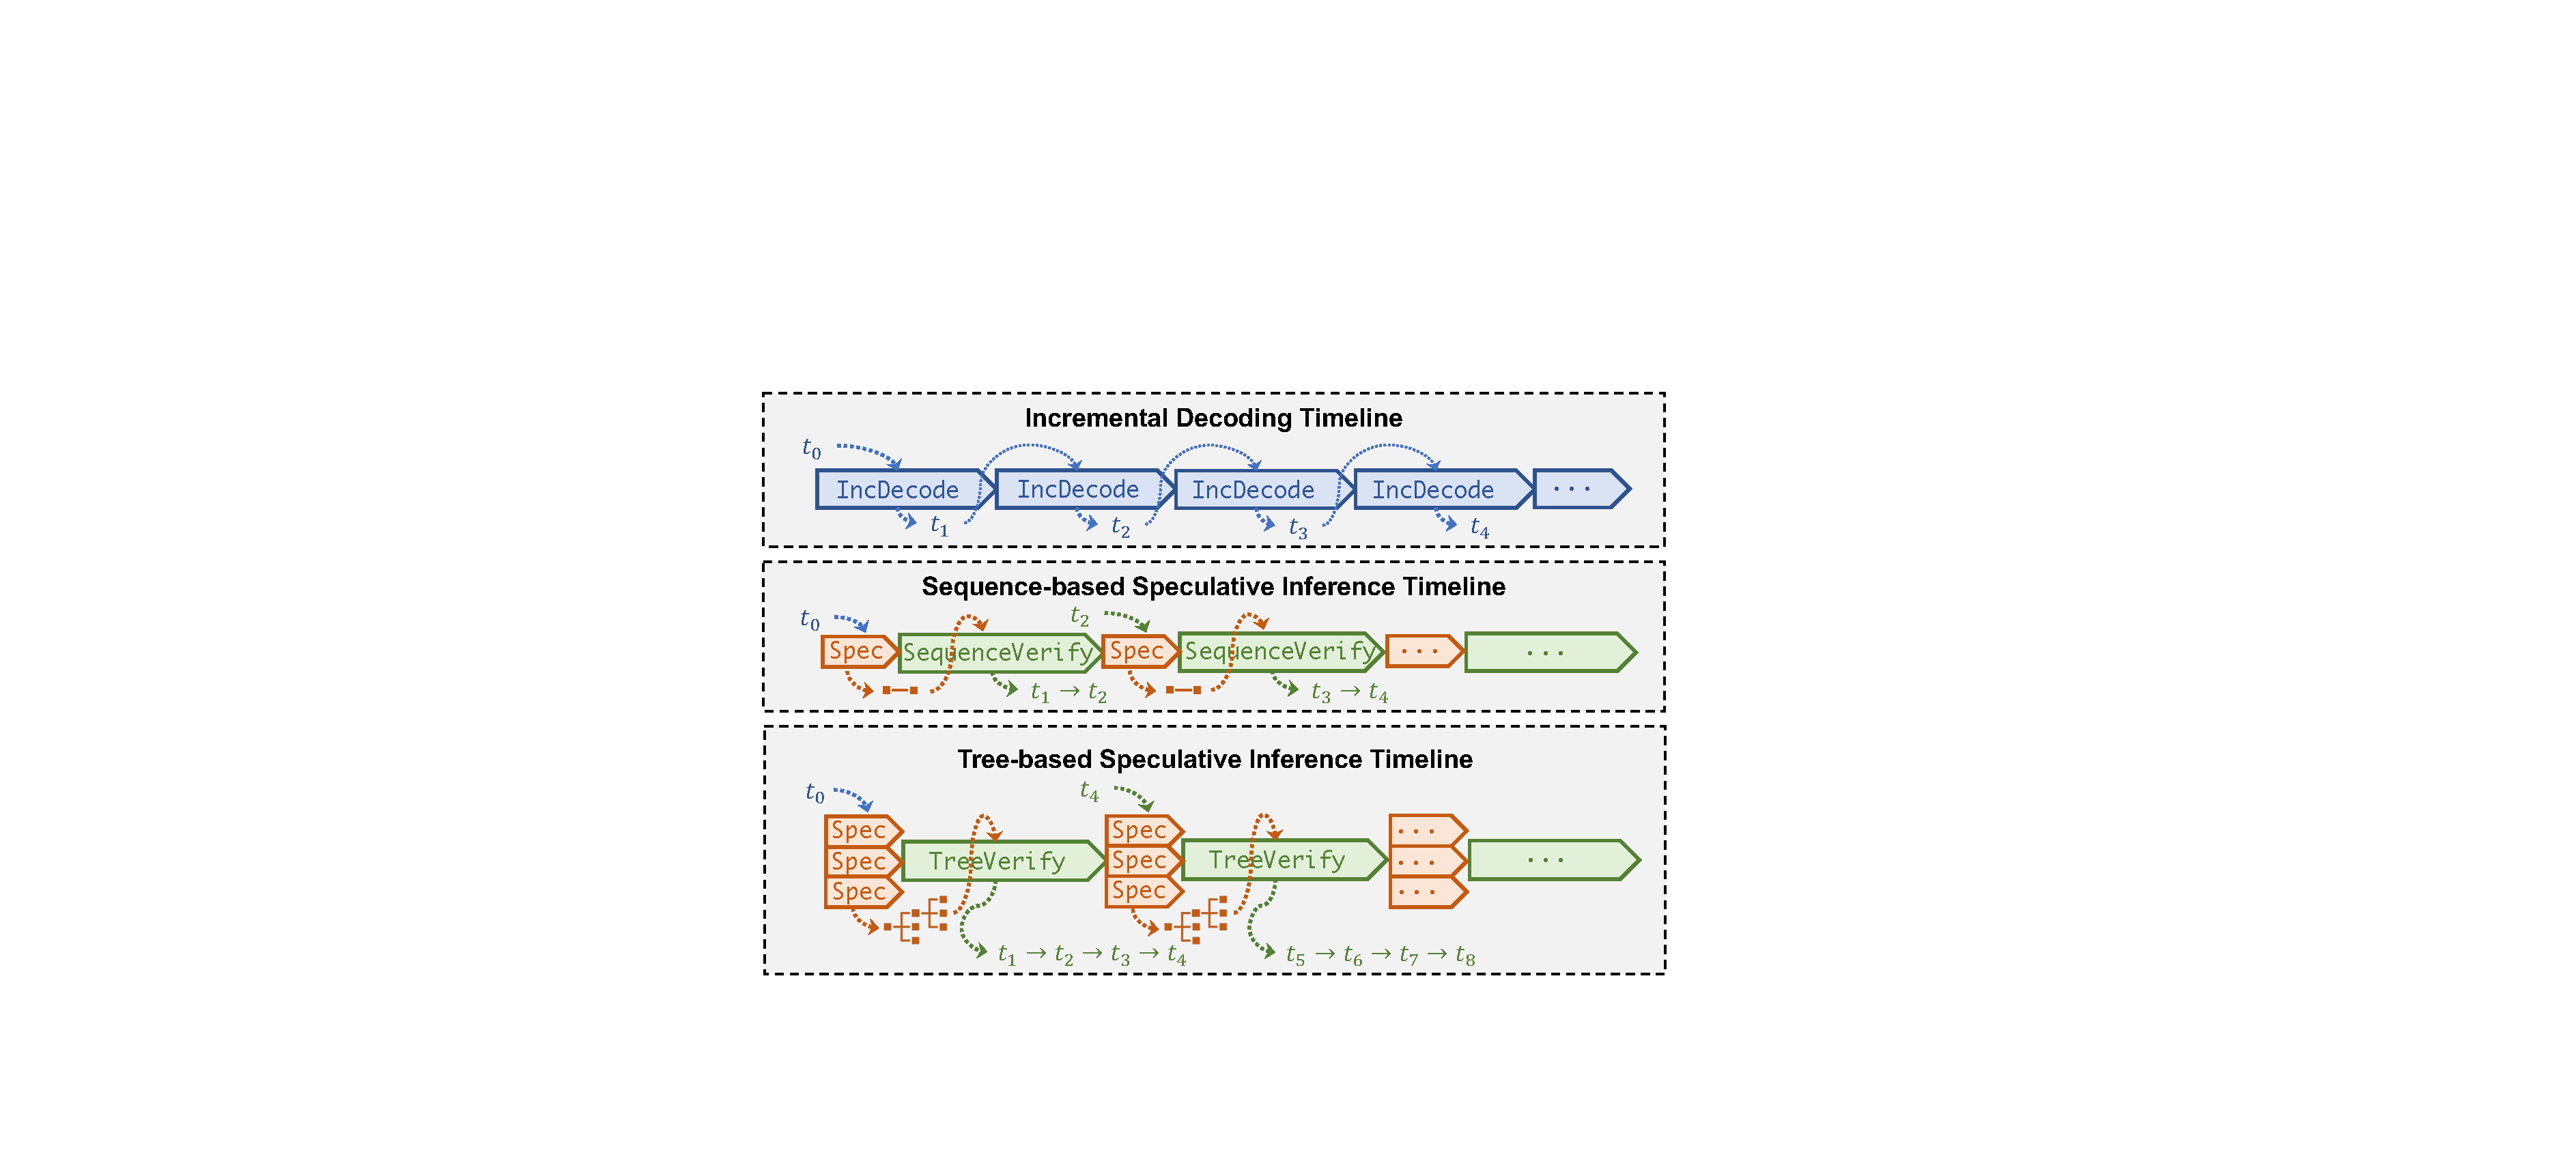
\includegraphics[width=\linewidth]{figures/specinfer/existing_overview6b6}
        \caption{Timeline comparison.}
        \label{background:fig:decoding:timeline}
    \end{subfigure}
    \caption{Incremental (autoregressive) decoding generates one token per forward pass of the LLM (a). Speculative decoding instead uses a cheap drafter to propose several tokens and verifies them against the LLM in a single pass; sequence-based speculation verifies one candidate continuation, whereas tree-based speculation, introduced in \Cref{ch:specinfer}, verifies many at once (b).}
    \label{background:fig:decoding}
\end{figure}

\paragraph{The KV cache.}
The attention output for token $t$ depends on the keys and values of all tokens $j \le t$.
Recomputing those keys and values at every decode step would make the cost of generating a sequence quadratic in its length, so all serving systems \emph{cache} the per-layer keys and values of every processed token and append to this \emph{KV cache} as generation proceeds~\cite{pope2023efficiently,vllm}.
The cache turns each decode step into a cheap operation for the model's linear layers (one new row) but makes memory the binding constraint: for a model with $L$ layers, $H_{kv}$ key-value heads of dimension $d_h$, each token occupies $2 \cdot L \cdot H_{kv} \cdot d_h$ values (keys and values) in the cache, which for a 70B-parameter model in 16-bit precision is on the order of hundreds of kilobytes per token and tens of gigabytes for a batch of long requests.
The cache is also what makes long-context and agentic workloads, whose prompts routinely run to tens of thousands of tokens (\Cref{background:sec:agents}), expensive to serve concurrently: the number of requests that fit on a GPU is bounded by the memory left after the weights, and managing that memory well is one of the main contributions of modern serving systems (\Cref{background:sec:serving}).

\subsection{Why Decoding Underutilizes GPUs}
\label{background:subsec:memory_bound}

The decode phase is \emph{memory-bandwidth bound}.
Every decode step must read all $N$ model parameters from GPU high-bandwidth memory (HBM) once, regardless of how many requests are batched together, and it performs roughly $2N$ floating-point operations per request in the batch.
With a batch of $B$ requests the arithmetic intensity of the step is therefore about $B$ operations per parameter byte read (in 16-bit precision, $B/2$ FLOPs per byte).
In the roofline model~\cite{williams2009roofline}, a kernel is compute bound only when its arithmetic intensity exceeds the ratio of peak compute to peak memory bandwidth of the device.
For an NVIDIA A100 (312 TFLOP/s of 16-bit tensor-core compute, 2 TB/s of HBM bandwidth) that ratio is about 150 FLOPs per byte, and for an H100 (roughly 1 PFLOP/s and 3.35 TB/s~\cite{nvidia2022hopper}) it is about 300.
Decode steps with batches of a few dozen requests, which is what latency targets usually allow, sit far below these ridge points: the tensor cores idle while the memory system streams weights, and the KV cache reads for long sequences add to the traffic without adding useful compute.
Prefill, with hundreds or thousands of tokens per request, sits on the other side of the ridge.

The consequence is that the latency of a decode step is close to the time to read the weights (and the KV cache) from HBM, and the GPU's compute capacity is mostly wasted during generation.
This observation is the premise of speculative decoding (\Cref{background:sec:specdec}): if a step is going to read all of the weights anyway, verifying several candidate tokens in that same step costs little more than generating one, so the ``free'' compute can be spent on checking guesses about the future~\cite{leviathan2022fast,chen2023accelerating,specinfer}.
It is also the premise of co-serving (\Cref{background:sec:peft}): the compute left idle by latency-critical decoding can be reclaimed by throughput-oriented work that shares the same weights.

\subsection{The Cost of Scale}
\label{background:subsec:cost}

Model quality has improved with scale~\cite{kaplan2020scaling,brown2020language,chowdhery2022palm}, and the cost of inference has grown with it.
GPT-3's 175 billion parameters require more than eight 40GB A100 GPUs just to hold the weights in half precision~\cite{brown2020language,zhang2022opt}; the open-weight DeepSeek-V3 has 671 billion parameters~\cite{deepseekai2024deepseekv3}; and frontier proprietary models~\cite{openai2023gpt4,gpt5} are larger still.
A single request to such a model takes seconds to serve, and a multi-GPU server costs hundreds of thousands of dollars and consumes kilowatts of power, with individual accelerators now exceeding 1,000W~\cite{lithos2025}.
Reasoning models that generate long chains of thought before answering~\cite{o1-preview,guo2025deepseek} multiply the number of decode steps per request, and agentic applications multiply the number of requests per task (\Cref{background:sec:agents}).
Serving efficiency is therefore not a second-order concern: it determines which models can be deployed at all, which applications are affordable, and how much latency a user experiences.
The systems in this thesis address this cost at three levels: by reducing the number of sequential decode steps (\Cref{ch:specinfer,ch:suffixdecoding}), by reclaiming the GPU capacity that bursty inference leaves idle (\Cref{ch:flexllm}), and by producing better kernels for the operators every step executes (\Cref{ch:fastkernels,ch:kernelseek}).

\section{LLM Serving Systems}
\label{background:sec:serving}

An LLM serving system accepts a stream of generation requests, schedules them onto one or more GPUs, and returns their outputs under latency and throughput constraints.
This section reviews the mechanisms that production systems use to do this efficiently, because they are both the foundation that the systems in this thesis are built on and the baselines they are compared against: \SpecInfer (\Cref{ch:specinfer}) is evaluated against vLLM, HuggingFace TGI, FasterTransformer, and FlexGen; \SuffixDecoding (\Cref{ch:suffixdecoding}) is implemented inside vLLM; \FlexLLM (\Cref{ch:flexllm}) is compared against dedicated vLLM inference clusters and PEFT finetuning stacks; and \FastKernels (\Cref{ch:fastkernels}) validates its measurement instrument against vLLM and SGLang before scoring any agent.

\subsection{Batching}
\label{background:subsec:batching}

Because a decode step is bandwidth bound, batching requests is the single most effective way to raise throughput: the weights are read once per step regardless of batch size, so adding a request to a batch adds compute but almost no memory traffic until the batch reaches the ridge point of \Cref{background:subsec:memory_bound}.
Early serving systems such as FasterTransformer~\cite{fastertransformer} batched at the granularity of requests, which forces the whole batch to wait for its longest member and leaves slots idle as shorter requests finish.
Orca~\cite{yu2022orca} introduced \emph{iteration-level scheduling} (now usually called \emph{continuous batching}), in which the scheduler revisits the batch at every decode step, retiring finished requests and admitting new ones immediately, together with \emph{selective batching} that batches the linear layers across requests while running attention per request.
Continuous batching is now universal: vLLM~\cite{vllm}, TGI~\cite{huggingface_tgi}, TensorRT-LLM~\cite{tensorrt-llm}, DeepSpeed-MII~\cite{deepspeed-mii}, and SGLang~\cite{sglang} all implement it.
Sarathi and Sarathi-Serve~\cite{agrawal2023sarathi,agrawal2024taming} refined it with \emph{chunked prefill}, which splits long prompts into chunks and co-schedules each chunk with the decode steps of other requests, so that a long prefill does not stall every in-flight request for an entire step.
NanoFlow~\cite{nanoflow} goes further and overlaps compute-, memory-, and network-bound operations within a single device by splitting the batch into nano-batches.
Throughout this thesis, iteration-level scheduling is the unit at which our systems make decisions: \SpecInfer and \SuffixDecoding change what one iteration verifies, and \FlexLLM changes what one iteration contains.

\subsection{Memory Management}
\label{background:subsec:memory}

With weights fixed, the KV cache determines how many requests can be batched.
vLLM's PagedAttention~\cite{vllm} applies virtual-memory ideas to this cache: instead of reserving a contiguous region sized for the maximum output length of each request, it allocates fixed-size blocks on demand and keeps a per-request block table, which eliminates most of the internal and external fragmentation of earlier systems and lets blocks be shared between requests with a common prefix (for example, parallel samples from the same prompt).
SGLang's RadixAttention~\cite{sglang} generalizes prefix sharing across requests over time by keeping the KV cache of recently served prompts in a radix tree keyed by token sequence, so that a new request that shares a prefix with an earlier one (the system prompt of a chat application, the few-shot examples of a pipeline, the accumulated transcript of an agent) skips prefill for the shared portion; SGLang pairs this with a frontend language for expressing multi-call LLM programs and a compressed finite-state machine for constrained decoding.
Prefix caching is highly relevant to the agentic workloads of \Cref{background:sec:agents}, which reuse context aggressively; \SuffixDecoding (\Cref{ch:suffixdecoding}) exploits the complementary observation that such workloads also repeat their \emph{outputs}.

\subsection{Multi-GPU Serving}
\label{background:subsec:parallelism}

Models that do not fit on one GPU, or whose latency targets cannot be met by one GPU's bandwidth, are served across several.
\emph{Tensor model parallelism}~\cite{shoeybi2020megatronlm} partitions the weight matrices of each layer across GPUs, so every GPU holds a slice of every layer and the GPUs exchange partial results with an all-reduce after each attention and FFN block; it divides the per-step weight read across devices, directly lowering decode latency, but requires fast interconnect (NVLink) and is therefore usually confined to a single node.
\emph{Pipeline parallelism}~\cite{huang2019gpipe} instead assigns contiguous groups of layers to different GPUs and streams micro-batches through them; it needs only point-to-point communication and scales across nodes, but does not reduce the latency of a single request and introduces pipeline bubbles.
Production systems combine the two, with tensor parallelism within a node and pipeline parallelism across nodes~\cite{aminabadi2022deepspeed,tensorrt-llm}, and this is also the configuration used in \SpecInfer's distributed experiments (\Cref{ch:specinfer}).
Choosing a parallelization strategy is itself an optimization problem; FlexFlow and Unity~\cite{jia2019flexflow,unger2022unity} and Alpa~\cite{zheng22-alpa} search this space automatically for training, AlpaServe~\cite{li2023alpaserve} does so for serving multiple models, and \FlexLLM extends the idea with \emph{dependent parallelization} of PEFT adapters relative to the base model they attach to (\Cref{ch:flexllm}).
More recent work disaggregates the prefill and decode phases onto separate GPU pools so that each can be provisioned and parallelized for its own profile~\cite{zhong2024distserve,patel2024splitwise}.

\paragraph{Offloading.}
At the other end of the spectrum, \emph{offloading-based} inference serves a model that does not fit in GPU memory from a single commodity GPU by keeping weights, KV cache, or both in CPU DRAM or on disk and streaming them to the GPU as needed~\cite{sheng2023flexgen,aminabadi2022deepspeed}.
FlexGen~\cite{sheng2023flexgen} formulates the placement and schedule as a linear program and reaches high throughput by processing very large batches between transfers, but each decode step still pays the cost of moving the weights over PCIe, which is an order of magnitude slower than HBM.
Offloading magnifies the memory-bound character of decoding: anything that extracts more than one token from each pass over the weights, as speculative decoding does, pays off proportionally more, which is why \SpecInfer's gains are largest in the offloading setting (\Cref{ch:specinfer}).

\subsection{Service-Level Objectives and Workloads}
\label{background:subsec:slo}

Serving systems are evaluated against \emph{service-level objectives} (SLOs) that reflect how users experience generation~\cite{zhong2024distserve,wang2024towards,adaserve}.
\emph{Time to first token} (TTFT) is the latency of prefill plus queueing; \emph{time per output token} (TPOT), or per-token latency, is the interval between successive output tokens during decode; and end-to-end latency is their combination over the length of the output.
Interactive chat tolerates a TPOT of a few tens of milliseconds, while agentic pipelines care about the end-to-end latency of an entire multi-call task (\Cref{background:sec:agents}).
Throughput, measured in requests or tokens per second, is the system-level counterpart, and \emph{goodput}, the throughput of requests that meet their SLOs, combines the two~\cite{zhong2024distserve,turbospec}.
A system can trade these against each other: larger batches raise throughput but lengthen each decode step and hence TPOT, so a latency SLO caps the usable batch size and, by \Cref{background:subsec:memory_bound}, caps GPU utilization.

Real inference traffic complicates the picture further.
Production traces show request arrivals that are bursty and non-stationary over minutes and hours, with prompt and output lengths that vary by orders of magnitude across and within applications~\cite{wang2024towards,burstgpt}.
Because the latency SLO must hold during bursts, operators provision for peaks, and the GPUs sit partially idle the rest of the time; reported average utilizations of production inference clusters are as low as 52\% at Microsoft and 10\% at Alibaba~\cite{lithos2025}.
Work on spot instances~\cite{miao2023spotserve}, fair scheduling across tenants~\cite{sheng2024fairness,aqua2024}, and SLO-aware speculation~\cite{adaserve,turbospec} all respond to this variability.
\FlexLLM (\Cref{ch:flexllm}) takes the complementary view that the idle capacity reserved for bursts should be filled by work that tolerates delay, and it does so at the granularity of individual tokens within an iteration so that it can give the capacity back the moment a burst arrives.

\section{Speculative Decoding}
\label{background:sec:specdec}

\subsection{Draft and Verify}
\label{background:subsec:draft_verify}

Speculative decoding exploits the asymmetry identified in \Cref{background:subsec:memory_bound}: an LLM can only \emph{generate} one token per forward pass, but it can \emph{verify} many.
The idea is borrowed from speculative execution in processors, where a pipeline predicts the outcome of a branch and executes ahead of it, discarding the work if the prediction turns out to be wrong~\cite{burton1985speculative,gabbay1996speculative,smith1998study,hennessy2011computer}.
In the LLM setting~\cite{stern2018blockwise,leviathan2022fast,chen2023accelerating,xiaspeculative,gante2023assisted}, a cheap \emph{drafter} proposes a sequence of $\gamma$ candidate tokens $\hat{x}_{t+1}, \ldots, \hat{x}_{t+\gamma}$ given the prefix $x_{\le t}$.
The target LLM then runs a single forward pass over the prefix extended by the candidates, which yields its next-token distribution at every one of the $\gamma + 1$ positions simultaneously, exactly as a prefill pass does.
A \emph{verifier} walks the candidates in order, accepting each token that the target model agrees with and stopping at the first disagreement; the position at which it stops also provides a correctly distributed token from the target model, so every verification step produces at least one new token and at most $\gamma + 1$.
\Cref{background:fig:decoding:timeline} contrasts this with incremental decoding.
When the drafter is cheap and its proposals are frequently accepted, the number of expensive sequential passes over the target model shrinks by the average number of accepted tokens, and because each pass reads the weights once regardless of how many positions it evaluates, the extra compute of verification is nearly free while decode stays memory bound.

\subsection{Lossless Verification}
\label{background:subsec:lossless}

What distinguishes speculative decoding from lossy acceleration techniques such as quantization or pruning~\cite{frantar2023gptq,frantar2023sparsegpt,biglittletransformer} is that it provably preserves the output distribution of the target model.
Under greedy decoding the argument is immediate: the verifier accepts a candidate only if it equals the target model's argmax at that position, so the accepted prefix is exactly what incremental greedy decoding would have produced, and the first rejected position is replaced by the target's own argmax.
Under stochastic decoding the guarantee comes from \emph{speculative sampling}~\cite{leviathan2022fast,chen2023accelerating}.
Let $p(\cdot)$ be the target distribution at a position and $q(\cdot)$ the drafter's distribution, and let $\hat{x} \sim q$ be the candidate.
The verifier accepts $\hat{x}$ with probability $\min\!\big(1, p(\hat{x})/q(\hat{x})\big)$; on rejection it samples a replacement from the residual distribution
\[
p'(x) = \frac{\max\big(0,\, p(x) - q(x)\big)}{\sum_{x'} \max\big(0,\, p(x') - q(x')\big)}
\]
and stops.
A short calculation shows that the token emitted at that position, whether accepted or resampled, is distributed exactly according to $p$, independently of $q$.
The drafter therefore affects only \emph{speed}, through how often its candidates are accepted, and never \emph{quality}; a bad drafter degrades gracefully to incremental decoding.
This property is what makes speculative decoding safe to deploy transparently in a serving system, and both \SpecInfer and \SuffixDecoding preserve it: \SpecInfer extends speculative sampling to token trees with its multi-step speculative sampling (\Cref{ch:specinfer}), and \SuffixDecoding inherits the greedy and stochastic guarantees unchanged because its drafter, though not a model, produces candidates that are verified the same way (\Cref{ch:suffixdecoding}).

\subsection{Sequence-Based and Tree-Based Speculation}
\label{background:subsec:tree}

The original formulation drafts a single sequence.
Its expected gain per step is governed by the acceptance rate $\alpha$: if each candidate is accepted independently with probability $\alpha$, the expected number of tokens per verification step is $(1 - \alpha^{\gamma+1})/(1 - \alpha)$~\cite{leviathan2022fast}, which saturates quickly for moderate $\alpha$ because a single early mistake wastes every candidate after it.
Drafters that are small enough to be cheap are often 100--1000$\times$ smaller than the target and frequently disagree with it, particularly under stochastic decoding, where even a well-aligned drafter guesses the sampled token only with the probability the target assigns to it.

\emph{Tree-based speculation}, introduced by \SpecInfer~\cite{specinfer} and adopted since by most model-based methods~\cite{cai2024medusasimplellminference,li2024eagle,eagle2,sequoia}, replaces the single draft sequence with a \emph{token tree} in which each node is a candidate token and each root-to-node path is a candidate continuation.
The tree hedges the drafter's uncertainty: where a sequence commits to one guess at every position, a tree can keep several alternatives at the positions where the drafter is unsure, so that a mistake on one branch does not forfeit the tokens on another.
Verifying a tree in one forward pass requires an attention variant that respects the tree's ancestor structure rather than a linear causal mask, a \emph{tree attention} in which each node attends only to its ancestors, plus a KV-cache layout that stores the tree's branches without duplicating their shared prefix.
\SpecInfer's tree-based parallel decoding provides exactly this, and it raises the per-token verification success rate from 52--57\% for a single sequence to 96--97\% for a tree in its stochastic-decoding experiments (\Cref{ch:specinfer}).
Later work optimizes the \emph{shape} of the tree: Sequoia~\cite{sequoia} chooses a topology for a given hardware budget, EAGLE-2~\cite{eagle2} grows the tree dynamically according to the drafter's confidence, and SLO-aware schedulers size the tree per request~\cite{adaserve}.

\subsection{Model-Based and Model-Free Drafters}
\label{background:subsec:drafters}

Drafters divide into two families according to where their predictions come from.

\paragraph{Model-based drafters} run a neural network.
The simplest is a small language model from the same family as the target, such as OPT-125M for OPT-175B or LLaMA-68M for LLaMA-65B~\cite{leviathan2022fast,chen2023accelerating,specinfer}; \SpecInfer additionally fine-tunes several such small models jointly so that their proposals cover complementary parts of the target's output (\Cref{ch:specinfer}).
Medusa~\cite{cai2024medusasimplellminference} avoids a separate model by attaching extra decoding heads to the target that predict the tokens two, three, and more positions ahead from the current hidden state.
EAGLE~\cite{li2024eagle,eagle2,li2025eagle3scalinginferenceacceleration} trains a lightweight autoregressive head on the target's hidden features rather than its tokens, which removes most of the drafter's uncertainty and currently gives the highest acceptance rates among model-based methods.
Related approaches include blockwise parallel decoding~\cite{stern2018blockwise,kim2024accelerating}, multi-token prediction heads trained into the model~\cite{gloeckle2024multitoken}, self-speculation using early exits or skipped layers of the target~\cite{draftverify,bita}, and lookahead decoding, which generates n-grams in parallel with Jacobi iteration~\cite{fu2024lookahead}.
All of them spend GPU time on the drafter at every step, and that time is not negligible: a draft head or small model must itself be executed autoregressively to produce $\gamma$ tokens, it competes with the target for the GPU, and the two must be interleaved at the kernel level~\cite{sequoia,eagle2}.

\paragraph{Model-free drafters} look the candidates up instead of computing them.
Prompt lookup decoding~\cite{saxena2023prompt} searches the current prompt for the most recent occurrence of the last few generated tokens and proposes whatever followed it; LLMA~\cite{yang2023inference} does the same against retrieved reference documents, REST~\cite{he2024rest} against a datastore built from a corpus, Token Recycling~\cite{luo2024turningtrashtreasureaccelerating} against the target model's own recent top-$k$ predictions, and ANPD~\cite{ou2024losslessaccelerationlargelanguage} against an adaptive n-gram model of the prefix.
These drafters cost microseconds on the CPU and leave the GPU entirely to the target model, so their overhead is negligible; their acceptance rate, however, depends on how much of the output is literally present in their reference text.
In open-ended conversation this is little, and model-free methods lose to model-based ones; in workloads that copy, edit, or regenerate existing text, such as code editing and the agentic pipelines of \Cref{background:sec:agents}, long runs of output are predictable from context and lookup-based drafting can accept dozens of tokens at a time.
The methods above also typically speculate a \emph{fixed} number of tokens regardless of how likely they are to be accepted, which wastes verification compute when the match is weak.

\subsection{The Acceptance-Overhead Tradeoff}
\label{background:subsec:tradeoff}

The speedup of any speculative method is governed by two quantities: the expected number of accepted tokens per step, which depends on the drafter's alignment with the target and on the shape and length of the speculation, and the per-step overhead, which includes the drafter's own cost, the extra verification compute (significant once batches approach the ridge point, since verifying $\gamma + 1$ positions per request multiplies the batch's token count), and the serving system's orchestration.
Model-based drafters buy acceptance with overhead; model-free drafters have almost no overhead but only speculate well on repetitive text.
Longer speculation raises the ceiling but lowers the acceptance of the trailing tokens, and the optimal length shrinks as the batch grows~\cite{turbospec}.
A good speculative decoding system therefore has to be \emph{adaptive}: it should speculate aggressively when it is confident and conservatively otherwise, and it should fall back to incremental decoding when neither is warranted.

\paragraph{Positioning.}
\SpecInfer (\Cref{ch:specinfer}) is the model-based, tree-structured point in this design space: it introduces token trees and tree-based parallel decoding, shows how to build trees from one or several small speculative models, and proves that tree verification remains lossless under stochastic decoding.
\SuffixDecoding (\Cref{ch:suffixdecoding}) is the model-free point, specialized for agentic workloads: it drafts from suffix trees over the prompt and over previous outputs, uses frequency statistics in those trees to score candidates and to decide \emph{how far} to speculate at each step, and can hand over to a model-based drafter when the trees have nothing to offer.
Both leave the target model's output distribution untouched.

\section{Parameter-Efficient Finetuning and LLM Platforms}
\label{background:sec:peft}

\subsection{Finetuning as a Service}
\label{background:subsec:finetuning_service}

Pretraining an LLM is expensive enough that almost no organization does it, and a small number of foundation models are instead adapted to many downstream uses by \emph{finetuning}: continued training on a task-specific dataset~\cite{devlin2018bert,radford2019language,brown2020language,houlsby2019parameter,zhang2021share}.
Demand for finetuning comes from the need to customize models to a domain or style~\cite{liu2024customizing}, to train on private data without sharing it~\cite{tan2024democratizing}, and to keep models current as data changes~\cite{gao2023unified}.
Every major LLM platform therefore offers a finetuning API alongside its inference API~\cite{openaifinetuning,googlefinetuning,databricksfinetuning}, and open-source toolkits make the same workflow available on self-hosted clusters~\cite{peft,llamafactory,transformers}.
From the operator's point of view this creates two workloads with opposite characteristics over the same models: inference is latency-critical, bursty, and submitted by users one request at a time, whereas finetuning is throughput-oriented, tolerant of delays of minutes to hours, and submitted as a whole dataset at once.

\subsection{Parameter-Efficient Finetuning}
\label{background:subsec:peft_methods}

Full finetuning updates every parameter and so requires, per model copy, the memory for the weights, their gradients, and the optimizer state, several times the memory of inference~\cite{kingma2014adam}.
\emph{Parameter-efficient finetuning} (PEFT) methods~\cite{ding2023parameter} instead freeze the pretrained weights and train a small number of new or selected parameters.
Adapters~\cite{houlsby2019parameter,pfeiffer2020adapterfusion} insert small bottleneck layers between the frozen ones; prefix and prompt tuning~\cite{li2021prefix,lester2021power,liu2023gpt} learn virtual tokens prepended to the input or to each layer's keys and values; (IA)$^3$~\cite{liu2022few} learns per-dimension scaling vectors; and unified frameworks combine these by heuristics or architecture search~\cite{he2021towards,mao2021unipelt,zhou2023autopeft}.
The dominant method is \emph{low-rank adaptation} (LoRA)~\cite{hu2021lora}, which represents the update to a weight matrix $W \in \mathbb{R}^{d \times k}$ as the product of two low-rank factors, $W + BA$ with $B \in \mathbb{R}^{d \times r}$, $A \in \mathbb{R}^{r \times k}$, and $r \ll \min(d, k)$; the trainable parameters shrink by orders of magnitude, no new inference latency is introduced if $BA$ is merged into $W$, and QLoRA~\cite{dettmers2023qlora} extends the recipe to a 4-bit quantized base model so that large models can be finetuned on a single GPU.
PEFT reduces trainable parameters and optimizer state dramatically, but it does not by itself reduce the \emph{activation} memory of backpropagation, which training systems retain for every layer in order to compute gradients; \FlexLLM shows that for PEFT specifically, much of that activation memory is unnecessary because the frozen weights need no gradient, and it prunes the corresponding dependencies from the backward graph (\Cref{ch:flexllm}).

Two properties of PEFT matter for this thesis.
First, every finetuning job over a given base model, and every inference request against that base model or any of its finetuned variants, executes the \emph{same frozen forward computation}; the variants differ only in a small adapter applied on the side.
Second, the adapters are small enough that many of them can be resident on one GPU at the same time.
Together these make it possible to batch work from different adapters, and from different kinds of jobs, through a single copy of the base model.

\subsection{Multi-Adapter Serving}
\label{background:subsec:multi_adapter}

Serving systems have exploited the first property for inference.
PetS~\cite{zhou2022pets} decouples each linear layer into a shared base operation and small task-specific operations so that requests for different adapters share the base computation.
Punica~\cite{chen2023punica} introduces a segmented gather-matrix-vector CUDA kernel that applies different LoRA adapters to different requests within one batch, and S-LoRA~\cite{sheng2023s} adds unified paging of adapter weights and KV cache together with heterogeneous batching to serve thousands of adapters from one GPU.
dLoRA~\cite{wu2024dlora} dynamically switches between merged and unmerged adapter execution and migrates requests across replicas, Chameleon~\cite{iliakopoulou2024chameleon} caches and schedules adapters adaptively, and reports from practice show hundreds of task-specific LoRA models rivaling much larger general models at a fraction of the serving cost~\cite{zhao2024lora}.
These systems share base weights across inference requests for different adapters; \FlexLLM extends sharing in the other direction, across inference and \emph{finetuning} of adapters, where the forward pass is identical but the finetuning side also needs a backward pass.

\subsection{Separate Clusters and GPU Sharing}
\label{background:subsec:gpu_sharing}

Despite this sharing opportunity, the prevailing deployment pattern runs inference and finetuning on \emph{separate, dedicated clusters}, each with a system specialized for its workload~\cite{weng2022mlaas,gao2022deep,chen2023deepboot}.
The inference cluster is provisioned for peak load to protect its SLOs, and by \Cref{background:subsec:slo} it is underutilized most of the time; the finetuning cluster, meanwhile, cannot touch that idle capacity.
Reclaiming it requires sharing GPUs between the two workloads, and the systems literature offers three broad mechanisms~\cite{yu2022survey}.
\emph{Temporal sharing} time-slices a GPU between jobs; Gandiva~\cite{xiao2018gandiva} and AntMan~\cite{xiao2020antman} apply it to deep-learning training clusters, and PipeSwitch~\cite{bai2020pipeswitch} and PREMA~\cite{choi2020prema} reduce the cost of switching and preempting.
Time slicing lets each job use the whole GPU, but an inference request that arrives during a finetuning slice must wait for the slice to end, which is incompatible with millisecond latency targets unless the slices are very short, in which case switching overhead and the loss of batching dominate.
\emph{Spatial sharing} runs kernels from different jobs concurrently on disjoint subsets of the GPU's streaming multiprocessors, via multiple CUDA streams, NVIDIA's Multi-Process Service (MPS)~\cite{mps}, or the hardware partitioning of Multi-Instance GPU (MIG)~\cite{mig}; GSLICE~\cite{dhakal2020gslice}, Gpulet~\cite{choi2022serving}, and MuxFlow~\cite{zhao2023muxflow} build schedulers on top of these.
Spatial partitions, however, are coarse and slow to reconfigure (MIG partitions in particular cannot be resized without draining the GPU~\cite{migpartition}), so a partition sized for normal inference load fails during a burst while one sized for the burst wastes resources the rest of the time; and because the two jobs' kernels remain separate, each reads the shared base weights from HBM independently.
Across all of these mechanisms, prior work has found that co-locating training with inference degrades inference latency unless the system is carefully designed around it~\cite{romero2021infaas,choi2022serving}.

\paragraph{Positioning.}
\FlexLLM (\Cref{ch:flexllm}) introduces a fourth mechanism, \emph{co-serving}, that is specific to LLMs and PEFT.
Because inference requests and PEFT finetuning jobs over the same base model execute the same frozen forward computation, \FlexLLM fuses them at the granularity of individual tokens within one iteration-level batch: finetuning tokens ride along in the same GPU kernels as inference tokens, the weights are read once for both, and a token-level scheduler decides at every iteration how many finetuning tokens to admit given the current inference load and its SLO.
Reallocation therefore happens at the millisecond timescale of an iteration rather than at the timescale of a time slice or a partition change, which is what allows the system to absorb inference bursts without violating SLOs while filling the troughs with finetuning.

\section{Agentic LLM Workloads}
\label{background:sec:agents}

\subsection{What Agents Are}
\label{background:subsec:agents_def}

An \emph{agentic} application does not issue a single prompt and return a single completion; it decomposes a task into many LLM calls whose inputs depend on the outputs of earlier calls and on the results of actions taken in an environment.
The building blocks are by now well established.
Chain-of-thought prompting~\cite{wei2022chain} has the model reason step by step before answering, and reasoning models train this behavior in~\cite{o1-preview,guo2025deepseek}.
ReAct~\cite{yao2023react} interleaves reasoning with \emph{tool use}: the model emits an action (a search query, a shell command, a function call), the harness executes it and appends the observation to the context, and the model continues.
\emph{Self-consistency}~\cite{wang2023selfconsistencyimproveschainthought} samples several reasoning paths for the same prompt and votes; \emph{self-refinement} and Reflexion~\cite{madaan2023selfrefine,shinn2023reflexion} have the model critique and revise its own output over several rounds; decomposed prompting~\cite{khot2023decomposedpromptingmodularapproach} splits a task into subtasks handled by specialized prompts; and \emph{multi-agent} frameworks~\cite{wu2023autogen,chen2024autoagentsframeworkautomaticagent,wang2024mixtureofagentsenhanceslargelanguage} assign roles to several model instances that exchange messages.
Retrieval-augmented generation~\cite{gao2024retrievalaugmentedgenerationlargelanguage,wang2024speculativeragenhancingretrieval} adds retrieved documents to the context of some or all calls.
A production pipeline such as the AgenticSQL system evaluated in \Cref{ch:suffixdecoding} composes several of these: a classification call, parallel candidate-generation calls, a merge call, and refinement calls, all for one user question.

\paragraph{Software-engineering agents.}
The most demanding and most studied agentic workload is software engineering.
Given a repository and an issue description, an agent must navigate the code, reproduce the problem, edit files, run tests, and iterate until the tests pass.
SWE-bench~\cite{jimenez2024swebenchlanguagemodelsresolve} made this measurable with real GitHub issues and their test suites, and a succession of agents has driven resolution rates up: SWE-agent~\cite{yang2024sweagent} showed that the design of the agent-computer interface (how files are viewed, searched, and edited) matters as much as the model; CodeAct and OpenHands~\cite{wang2024executablecodeactionselicit,openhands} let the agent act by writing and executing code; Agentless~\cite{xia2024agentless} showed that a fixed localize-repair-validate pipeline is competitive with free-form agents; and commercial harnesses such as Claude Code and Codex~\cite{anthropic2025claudecode,codex} now run such loops at scale.
An agent of this kind issues tens to hundreds of LLM calls for one task, each with the accumulated transcript of previous calls in its context, and each separated from the next by the execution of a tool.

\subsection{Why Agents Stress Serving Systems}
\label{background:subsec:agents_stress}

Agentic workloads differ from chat in ways that invalidate several assumptions of the systems in \Cref{background:sec:serving}.

\paragraph{Many dependent calls.}
A task is not done until its last call returns, and the calls are sequentially dependent, so per-call latency accumulates: a pipeline of 50 dependent calls at 2 seconds each takes nearly two minutes regardless of throughput.
Per-token decode latency, which chat tolerates because humans read slowly, becomes the dominant term in end-to-end task time, which is what \Cref{ch:suffixdecoding} measures.
Systems such as Parrot~\cite{lin2024parrot}, ALTO~\cite{10.1145/3642970.3655844}, and Autellix~\cite{luo2025autellix} expose the structure of the program to the serving system so that it can schedule across calls, pipeline between agents, and prioritize calls on the critical path, and Dynasor~\cite{fu2024efficientlyservingllmreasoning} terminates reasoning paths early once their outcome is certain.

\paragraph{Long contexts.}
Each call carries the transcript so far: the system prompt, tool definitions, the issue, every file the agent has viewed, and every command output.
Contexts of tens of thousands of tokens are routine, so the KV cache of \Cref{background:subsec:autoregressive} grows large, prefill is repeated for mostly-unchanged prompts unless prefix caching (\Cref{background:subsec:memory}) catches it, and the number of concurrent agents a GPU can host shrinks.

\paragraph{Heavy repetition.}
Consecutive calls of an agent overlap not only in their prompts but in their \emph{outputs}.
A self-refinement loop rewrites a document while changing a few lines; a coding agent regenerates a function with one fix; a multi-agent pipeline produces structured outputs with the same schema and boilerplate every time; self-consistency samples share long stretches of reasoning; and SWE-bench agents repeatedly emit near-identical commands, file paths, and edit blocks.
This repetition is invisible to a model-based drafter, which must rediscover it token by token, but it is exactly what a model-free drafter can exploit.
Measured as the empirical entropy of the next token given a short context, agentic outputs are far more predictable than open-ended chat (\Cref{ch:suffixdecoding}).

\paragraph{Positioning.}
\SuffixDecoding (\Cref{ch:suffixdecoding}) targets this workload directly: it treats the outputs of earlier calls as a cache for drafting the outputs of later ones, maintains that cache in suffix trees that grow with the workload, and adapts its speculation length to how well the current context matches history, which pays off most on the long repeated runs that agents produce.
Agentic workloads also motivate the second half of this thesis in a different way.
The same coding agents that stress serving systems are now capable of writing systems code themselves, including the GPU kernels that serving systems depend on (\Cref{background:sec:kernelagents}).
\Cref{ch:fastkernels,ch:kernelseek} ask how well they do so under production conditions and how they should be steered when the kernel is hard.

\section{GPU Kernels for Machine Learning}
\label{background:sec:gpu}

\subsection{The GPU Execution Model}
\label{background:subsec:gpu_model}

Every operator in \Cref{background:sec:llm}, and every scheduling decision in \Cref{background:sec:serving,background:sec:peft}, ultimately executes as a sequence of GPU \emph{kernels}: functions launched over a grid of thread blocks, each block running on one of the GPU's \emph{streaming multiprocessors} (SMs)~\cite{nvidia2025cudaguide}.
An NVIDIA H100 has 132 SMs and a B200 has 148~\cite{nvidia2022hopper,nvidia2024blackwell}.
Threads execute in \emph{warps} of 32 that issue instructions in lockstep; a block's warps share a fast, software-managed \emph{shared memory} (up to 228KB per SM on Hopper) and a large register file, and the SM's warp schedulers hide latency by switching among resident warps.
The memory hierarchy below that is a shared L2 cache (50MB on H100) and HBM, whose bandwidth, 3.35TB/s on H100 and about 8TB/s on B200, is the resource that decode-phase kernels are bound by (\Cref{background:subsec:memory_bound}).
\emph{Tensor cores} perform dense matrix multiply-accumulate on small tiles at throughputs an order of magnitude above the general-purpose cores; on Hopper they are driven by warp-group-level asynchronous instructions (\texttt{wgmma}) whose operands live in shared memory, and on Blackwell by a new generation (\texttt{tcgen05}) that accumulates into a dedicated tensor memory, with cluster-level multicast and lower-precision formats added in each generation~\cite{nvidia2022hopper,nvidia2024blackwell}.
Hopper also introduced the \emph{Tensor Memory Accelerator} (TMA), which copies tiles between HBM and shared memory asynchronously, and thread-block clusters that let SMs share data through distributed shared memory.
Each of these features is exposed to the programmer, and each must be used explicitly to reach the hardware's peak.

\subsection{What Makes a Kernel Fast}
\label{background:subsec:kernel_fast}

The roofline model~\cite{williams2009roofline} gives the first-order answer: a kernel is limited either by memory bandwidth or by compute, and a fast kernel for a memory-bound operator moves the minimum number of bytes while a fast kernel for a compute-bound operator keeps the tensor cores busy.
Getting there involves a small set of recurring techniques, and the difficulty is in composing them.
\emph{Tiling} partitions the output into blocks sized so that the operands of each block fit in shared memory and registers, so that each byte loaded from HBM is reused many times; the choice of tile shape trades reuse against parallelism and register pressure.
\emph{Fusion} merges consecutive operators into one kernel so that intermediates never round-trip through HBM; FlashAttention~\cite{flashattention} is the canonical example, computing softmax attention tile by tile with an online normalization so that the $n \times n$ attention matrix is never materialized, which turns attention from memory bound to compute bound and makes long contexts feasible.
\emph{Occupancy}, the number of warps resident per SM, must be high enough to hide memory and pipeline latency but is capped by the registers and shared memory each block consumes.
\emph{Coalescing} arranges each warp's memory accesses to fall in contiguous, aligned segments so that one transaction serves 32 threads; tensor layouts in shared memory must additionally be \emph{swizzled} to avoid bank conflicts.
\emph{Overlap} keeps the memory system and the tensor cores busy simultaneously through software pipelining, multi-stage buffers, and, on recent GPUs, \emph{warp specialization}, in which producer warps issue asynchronous TMA loads while consumer warps run tensor-core instructions, synchronized through barrier phases~\cite{shah2024flashattention3}.
\emph{Persistent} kernels launch one block per SM that loops over work items, which amortizes launch cost and enables cross-tile scheduling, and on the host side, launch overhead, CUDA-graph capture, and the shape of the dispatch path can matter as much as the kernel body when the operator is small~\cite{hu2024korch,jin2026eventtensor}.
Public worklogs that take a matrix multiplication from a naive kernel to cuBLAS parity on Ampere, Hopper, and Blackwell~\cite{boehm2022cudammm,shankhdhar2024h100,modular2025blackwell} illustrate how many of these steps are needed and how the right sequence changes from one generation to the next.

\subsection{Programming Layers}
\label{background:subsec:programming_layers}

Kernels are written at several levels of abstraction, and the level determines how much of the machinery above the programmer controls.
At the bottom, CUDA C++~\cite{nvidia2025cudaguide} exposes threads, shared memory, and (through PTX intrinsics) every hardware feature; it offers the highest ceiling and the most ways to be wrong.
CUTLASS and its CuTe layout algebra~\cite{nvidia2023cutlass} provide templated building blocks for tiled GEMM-like kernels on NVIDIA tensor cores, and ThunderKittens~\cite{spector2025thunderkittens} offers a smaller set of tile primitives with the same goal; both encode hardware-specific best practices that would otherwise be rediscovered per kernel, at the cost of large compile-time template surfaces and dependence on the library tracking each new GPU.
Triton~\cite{triton} raises the level to blocked programs in a Python DSL whose compiler handles memory coalescing, shared-memory allocation, and tensor-core instruction selection; it is the default path for custom kernels in PyTorch and the language most kernel-generation benchmarks target (\Cref{background:sec:kernelagents}).
Above that, compilers generate kernels from the model graph: PyTorch's \texttt{torch.compile}~\cite{ansel2024pytorch2,paszke2019pytorch} captures Python bytecode and lowers it through Inductor to Triton, TVM and Ansor~\cite{chen2018tvm,zheng2020ansor} search over loop schedules, and graph-level optimizers such as TASO, PET, and Mirage~\cite{jia2019taso,wang2021pet,wu2025mirage} search over algebraic rewrites of the computation, with Mirage extending the search into the kernel and thread-block levels.
Finally, hand-optimized libraries sit alongside these: cuBLAS and cuDNN~\cite{nvidia2025cublas,nvidia2025cudnn} for dense linear algebra and convolution, and for LLM serving specifically, FlashAttention and its successors~\cite{flashattention,dao2024flashattention2,shah2024flashattention3,zadouri2026flashattention4}, FlashInfer~\cite{ye2025flashinfer}, and the kernels shipped inside vLLM, SGLang, and TensorRT-LLM~\cite{vllm,sglang,tensorrt-llm}.
The kernels a production serving system actually runs are drawn from the top of this stack, and any new kernel, whether written by a person or an agent, must beat them to be worth deploying; this is the baseline \FastKernels measures against (\Cref{ch:fastkernels}).

\subsection{Hardware Churn and Emerging Operators}
\label{background:subsec:churn}

The tradeoffs above are not stable across GPU generations.
Each generation changes the tensor-core instruction set, the memory hierarchy, and the asynchronous machinery, so the best kernel for an operator must be rewritten.
Attention is the clearest case~\cite{miao2023towards}: FlashAttention on Ampere~\cite{flashattention,dao2024flashattention2} was followed by FlashAttention-3 on Hopper~\cite{shah2024flashattention3}, built around warp specialization, \texttt{wgmma}, TMA, and pingpong scheduling to overlap softmax with matrix multiplication, and then by FlashAttention-4 on Blackwell~\cite{zadouri2026flashattention4}, rebuilt again around \texttt{tcgen05} and tensor memory; each rewrite reported a 1.5--2$\times$ speedup over its predecessor on the new hardware, and each took an expert team months.
The same holds for GEMM, where even NVIDIA's own libraries sit well below the hardware's speed of light on many production shapes~\cite{solexecbench}, and the gap widens for operators that are not GEMMs.
The emerging operators of \Cref{background:subsec:transformer}, MoE routing and expert dispatch, linear-attention and state-space scans, gated delta rules, low-bit quantized GEMMs, speculative-decoding verification over token trees, and multimodal preprocessing, arrive in new models faster than hand-written kernels can follow, so they are typically served first by generic PyTorch implementations or by \texttt{torch.compile} output, at a fraction of attainable performance.
Production serving stacks therefore live in a permanent state of kernel debt: at any moment, some operators on some hardware have mature kernels and others do not, and the set changes every time a model family or a GPU is released.
This churn is the concrete form that the thesis statement's premise takes at the kernel layer, and it is what motivates using agents to write kernels.

\section{LLM Agents for Code and Kernel Generation}
\label{background:sec:kernelagents}

\subsection{Coding Agents and Harnesses}
\label{background:subsec:coding_agents}

LLMs trained on code~\cite{chen2021evaluating} became useful for software engineering once they were placed in a \emph{harness}: a loop that lets the model read and edit files, run compilers and tests, observe the results, and try again~\cite{yang2024sweagent,openhands,anthropic2025claudecode,codex}.
How the harness is built changes what the same model can do.
The agent-computer interface of SWE-agent~\cite{yang2024sweagent} and the minimal pipeline of Agentless~\cite{xia2024agentless} both improved results by changing what the model sees rather than the model itself; practitioner guidance favors simple, composable loops over elaborate scaffolds~\cite{anthropic2024effectiveagents}; and giving the model too many tools or too much context has measurable costs~\cite{langchain2025toolload,liu2024lost}.
A parallel literature documents how LLMs behave as optimizers over long horizons: they search greedily from their priors~\cite{redko2026priorknowledge}, anchor on the solution in the prompt~\cite{jones2022cognitivebiases}, explore poorly without intervention~\cite{krishnamurthy2024explore}, stop early after a run of failures~\cite{merouani2025compilot}, lock in to early decisions under iterative refinement~\cite{javaji2025turnwise}, and report success that the environment contradicts~\cite{advani2026falsesuccess}.
Intrinsic self-correction helps less than one would hope~\cite{huang2024cannotselfcorrect,sharma2024sycophancy}, whereas external feedback on a model's own code, particularly feedback that proposes structural changes the model did not consider, substantially raises repair success~\cite{olausson2024selfrepair,wang2024hypothesissearch}.
These findings frame the design question of \Cref{ch:kernelseek}: what should a human, or a harness, supply to a coding agent working on a hard optimization target.

\subsection{Kernel-Generation Benchmarks}
\label{background:subsec:kernel_benchmarks}

GPU kernels are an attractive target for coding agents because the goal is objective (the output must match a reference and run faster), the feedback is cheap (compile, test, time), and the expertise is scarce (\Cref{background:subsec:churn}).
KernelBench~\cite{kernelbench} established the evaluation format: a PyTorch reference module, a set of input shapes, and a score combining correctness and speedup over the reference, organized into levels from single operators to whole models drawn from an earlier generation of architectures.
Successors broadened the surface, with TritonBench and CUDABench~\cite{tritonbench,cudabench} for specific languages, BackendBench and MultiKernelBench~\cite{backendbench,multikernelbench} for more backends, KernelCraft, ComputeEval, and NPUEval~\cite{kernelcraft,nvidia2025computeeval,kalade2025npueval} for emerging hardware and robustness, FlashInfer-Bench~\cite{flashinferbench,xing2026flashinferbench} and KSearch~\cite{cao2026ksearch} for serving kernels inside an inference engine, SOL-ExecBench~\cite{solexecbench} for production shapes scored against speed-of-light bounds, and CommBench and ParallelKernelBench~\cite{commbench,parallelkernelbench} for multi-GPU communication.

The first generation of benchmarks also revealed systematic weaknesses.
Their inputs are synthetic, usually random tensors of fixed shape, so kernels are never tested on the data-dependent behavior (MoE routing skew, ragged batches, paged caches) that dominates in production.
Their baselines are weak: speedup over eager PyTorch, or at best \texttt{torch.compile}, is easy to obtain and says little about whether the kernel beats what vLLM or SGLang already ship.
Their scoring is vulnerable to \emph{reward hacking}: agents have learned to exploit loose numerical tolerances, timing harness quirks, caching across runs, and reference implementations that can be bypassed, which robust-kbench and KernelBench-Verified~\cite{robustkbench,zhang2026kernelbenchverified} document and partially repair.
And their tasks are isolated: a kernel is scored alone, on one GPU, behind a simplified interface, so a benchmark win need not survive integration into the compilation stacks, interfaces, and end-to-end execution paths of a real serving system.

\subsection{Kernel-Generation Agents}
\label{background:subsec:kernel_agents}

Agents for these benchmarks span a \emph{structure-freedom} axis.
\emph{Scripted} agents fix what the model does at each step: a generate-test-refine loop with a policy trained by reinforcement learning on kernel rewards (Kevin, CUDA-L1, KernelLLM, AutoTriton, QiMeng, DrKernel, CUDA-Agent~\cite{baronio2025kevin,li2025cudal1,kernelllm2025,li2025autotriton,zhu2026qimeng,drkernel,cudaagent2026}), a menu of optimizations keyed to profiler diagnostics (Autocomp, KernelPro~\cite{hong2025autocomp,kernelpro2026}), or a team of agents with fixed roles for planning, coding, profiling, and review (Astra, KernelAgent, CudaForge, GEAK, KDA, AKO, and others~\cite{wei2025astra,kernelagent,cudaforge,wang2025geak,kda,han2026kda,ako,kernelskill2026,luo2026houmao,sun2026kernelclaw}).
These are sample-efficient but encode what to try, and they fail where the script is wrong: Autocomp collapses without its menu~\cite{hong2025autocomp}, and RL loops competitive on single operators fail on fused models~\cite{drkernel,zhu2026qimeng,cudaagent2026}.
\emph{Open-ended} agents use the LLM as the mutation operator of an \emph{evolutionary search} over a population of programs, in the lineage of FunSearch and AlphaEvolve~\cite{romeraparedes2024funsearch,alphaevolve} and continued by OpenEvolve, ShinkaEvolve, EvoEngineer, CUCo, KernelFoundry, and TTT-Discover~\cite{openevolve,lange2025shinkaevolve,guo2025evoengineer,cuco2026,wiedemann2026kernelfoundry,yuksekgonul2026tttdiscover}; AVO~\cite{chen2026avo} makes a self-directed coding agent the variation operator, and Meta and Cursor with NVIDIA run such loops across whole kernel libraries~\cite{liao2025kernelevolve,kernelevolve,cursor2026multiagent}.
The freedom buys headline results, including gains over FlashAttention-4 and over AlphaEvolve's own FlashAttention baseline~\cite{chen2026avo,alphaevolve}, and is paid for in trials: hundreds of explored directions over days, a large fraction of incorrect candidates~\cite{guo2025evoengineer,cuco2026}, and edits that undo earlier edits~\cite{pelleriti2026evotrace}.
Orthogonal to this axis is how much the agent is \emph{equipped}: tool-rich agents hand the model parsed profiler output, documentation retrieval, reference implementations, and persistent knowledge stores~\cite{chen2026avo,han2026kda}, while minimal agents give it a shell and a goal.
The evidence that equipment is what is missing is weak; profiler and compiler output rarely supply the specific hypothesis the model lacks~\cite{redko2026priorknowledge}, and in the MLSys 2026 FlashInfer kernel contest, agents given expert direction beat the same agents running autonomously on every kernel~\cite{mlsys26contest,shui2026harness}.

\paragraph{Positioning.}
\FastKernels (\Cref{ch:fastkernels}) addresses the benchmark side.
It derives its tasks top-down from real model architectures so that every task has a production counterpart, matches the interfaces of the production modules so that generated kernels can be deployed as-is, captures real inputs so that data-dependent operators are tested on data they will see, scores candidates against the kernels production frameworks ship rather than against PyTorch, and evaluates every candidate end to end inside the model it came from, where interface mismatches and composition failures surface.
Its seed evaluation shows that kernel-level success barely predicts deployment, which is the gap the benchmark exists to measure.
\KernelSeek (\Cref{ch:kernelseek}) addresses the agent side for deep targets such as FlashAttention-class kernels, where whole-pipeline choreography rather than local edits determines performance.
It keeps the freedom of an open-ended coding agent, equips it minimally with a harness that verifies correctness and timing against a seed kernel, and supplies \emph{direction} at decision points through questions that name a hypothesis without giving an answer; the questions that recur harden into a bank the agent applies to itself, and the whole composes with evolutionary search.

\section{Summary}
\label{background:sec:summary}

The thread running through this chapter is that each layer of the LLM serving stack has an efficiency problem whose solution has historically required scarce expertise, and that each layer is moving.
Autoregressive decoding underutilizes GPUs because it is memory bound (\Cref{background:sec:llm}), and serving systems have developed elaborate batching, memory-management, and parallelization machinery around that fact (\Cref{background:sec:serving}).
Speculative decoding turns the idle compute into parallel verification without changing the model's outputs, and the design space of drafters and tree shapes is where \SpecInfer (\Cref{ch:specinfer}) and \SuffixDecoding (\Cref{ch:suffixdecoding}) sit (\Cref{background:sec:specdec}).
Finetuning and inference over shared frozen base models could share GPUs, but the available sharing mechanisms are too coarse for bursty, latency-critical inference, which \FlexLLM (\Cref{ch:flexllm}) resolves at token granularity (\Cref{background:sec:peft}).
Agentic applications multiply the calls, lengthen the contexts, and repeat the outputs that serving systems must handle, which \SuffixDecoding exploits, and the same agents are becoming capable of writing systems code (\Cref{background:sec:agents}).
At the bottom of the stack, GPU kernels determine the performance of every operator, and every new GPU generation and every new operator reopens the question of how to write them (\Cref{background:sec:gpu}); LLM agents are the newest tool for answering it, but the benchmarks that evaluate them have not reflected production, and the agents themselves struggle on deep targets (\Cref{background:sec:kernelagents}), which \FastKernels (\Cref{ch:fastkernels}) and \KernelSeek (\Cref{ch:kernelseek}) respectively address.
In each case, the thesis's response is the same: use smaller models, workload history, feedback-driven runtimes, or coding agents to automate an optimization that expert-only workflows cannot keep up with, while preserving the correctness guarantees and service-level objectives that production deployments require.
